\documentclass{ubicomp-ext}
\usepackage{libertine} % for the pretty dark-circle-enclosed numbers
\usepackage{tikz}
\usepackage{verbatim}

\usepackage{float}
\usepackage{listings}
\usepackage{multicol}
\usepackage{color}
\usepackage{minibox}
\usepackage{fancybox}
\usepackage{fontspec}
\usepackage{ifthen}
\usepackage{tikzscale}
\newfontfamily{\lstsansserif}[Scale=.7]{Arial}
\newfontfamily{\textlst}{Arial}
\definecolor{Lemon}{HTML}{FFFACD}
\newcounter{lstNoteCounter}
\newcommand{\lnnum}[1]
    {\ifthenelse{#1 =  1}{\libertineGlyph{uni2776}}
    {\ifthenelse{#1 =  2}{\libertineGlyph{uni2777}}
    {\ifthenelse{#1 =  3}{\libertineGlyph{uni2778}}
    {\ifthenelse{#1 =  4}{\libertineGlyph{uni2779}}
    {\ifthenelse{#1 =  5}{\libertineGlyph{uni277A}}
    {\ifthenelse{#1 =  6}{\libertineGlyph{uni277B}}
    {\ifthenelse{#1 =  7}{\libertineGlyph{uni277C}}
    {\ifthenelse{#1 =  8}{\libertineGlyph{uni277D}}
    {\ifthenelse{#1 =  9}{\libertineGlyph{uni277E}}
    {\ifthenelse{#1 = 10}{\libertineGlyph{uni277F}}
    {\ifthenelse{#1 = 11}{\libertineGlyph{uni24EB}}
    {\ifthenelse{#1 = 12}{\libertineGlyph{uni24EC}}
    {\ifthenelse{#1 = 13}{\libertineGlyph{uni24ED}}
    {\ifthenelse{#1 = 14}{\libertineGlyph{uni24EE}}
    {\ifthenelse{#1 = 15}{\libertineGlyph{uni24EF}}
    {\ifthenelse{#1 = 16}{\libertineGlyph{uni24F0}}
    {\ifthenelse{#1 = 17}{\libertineGlyph{uni24F1}}
    {\ifthenelse{#1 = 18}{\libertineGlyph{uni24F2}}
    {\ifthenelse{#1 = 19}{\libertineGlyph{uni24F3}}
    {\ifthenelse{#1 = 20}{\libertineGlyph{uni24F4}}
    {NUM TOO HIGH}}}}}}}}}}}}}}}}}}}}}


\newcommand{\lstref}[1]{\lnnum{\ref{#1}}}

\newcommand{\lstnote}[1] {
\label{#1}\vbox{\llap{{\lnnum{\ref{#1}}}\hskip 1em}}
}

\lstnewenvironment{csource}[1][]
{
 \setcounter{lstNoteCounter}{0}
 \lstset{basicstyle=\lstsansserif, frame=lines, framexleftmargin=0.5em,
            framexrightmargin=0.5em, backgroundcolor=\color{Lemon}, showstringspaces=false, escapeinside={(*@}{@*)}, #1}
}{}

\usetikzlibrary{shadows,arrows,calc}
% Define the layers to draw the diagram
\pgfdeclarelayer{background}
\pgfdeclarelayer{foreground}
\pgfsetlayers{background,main,foreground}
 
% Define block styles  
\tikzstyle{materia}=[draw, fill=blue!20, text width=5.0em, text centered,
  minimum height=1.5em,drop shadow]
\tikzstyle{context} = [materia, text width=5em, minimum width=0em,
  minimum height=3em, rounded corners, drop shadow]
\tikzstyle{texto} = [above, text width=15em]
\tikzstyle{linepart} = [draw, thick, color=black!50, -latex', dashed]
\tikzstyle{line} = [draw, thick, color=black!50, -latex']
\tikzstyle{ur}=[draw, text centered, minimum height=0.01em]
 
% Define distances for bordering
\newcommand{\blockdist}{1.3}
\newcommand{\edgedist}{1.5}

\newcommand{\context}[2]{node (c#1) [context]
  {\textbf{#2}}}

% Draw background
\newcommand{\background}[7]{%
  \begin{pgfonlayer}{background}
    % Left-top corner of the background rectangle
    \path (#1.west |- #2.north)+(-0.15,1.35) node (a1) {};
    % Right-bottom corner of the background rectanle
    \path (#3.east |- #4.south)+(+0.15,#7) node (a2) {};
    % Draw the background
    \path[fill=yellow!20,rounded corners, draw=black!50, dashed]
      (a1) rectangle (a2);
    \path (a1.east |- a1.south)+(2.75,-0.4) node (u1)[texto]
      {\textit{#5}};
    \path ($(a1.west) !.5! (a2.west)$)+(-2.1,0) node (u1)[rotate = 90, align = center, text width = 0, texto]
      {\scriptsize{#6}};
  \end{pgfonlayer}}

\newcommand{\transreceptor}[3]{%
  \path [linepart] (#1.east) -- node [above]
    {\scriptsize Transreceptor #2} (#3);}
% Please be sure that you have the dependencies (i.e., additional LaTeX packages) to compile this example.

\copyrightinfo{
  Copyright is held by the author/owner(s).\\
  {\emph{UbiComp '13 Adjunct}}, Sept 8-12, 2013, Zurich, Switzerland.\\
  ACM 978-1-4503-2139-6/13/09...\$15.00.
}

\title{Torwads Context-Oriented Programming in Wireless Sensor Networks}

\numberofauthors{2}
% Notice how author names are alternately typesetted to appear ordered in 2-column format;
% i.e., the first 4 autors on the first column and the other 4 auhors on the second column.
% Actually, it's up to you to strictly adhere to this author notation.
\author{
  \vspace{-1.5em} % lisatolles: The abstract heading should start at the time height on the page as the authors names
  \alignauthor{
  	\textbf{First Author}\\
  	\affaddr{AuthorCo, Inc.}\\
  	\affaddr{123 Author Ave.}\\
  	\affaddr{Authortown, PA 54321 USA}\\
  	\email{author1@anotherco.com}
  }\alignauthor{
  	\textbf{Fifth Author}\\
  	\affaddr{AuthorCo, Inc.}\\
  	\affaddr{123 Author Ave.}\\
  	\affaddr{Authortown, PA 54321 USA}\\
  	\email{author5@anotherco.com}
  }
  \vfil
}

% Paper metadata (use plain text, for PDF inclusion and later re-using, if desired)
\def\plaintitle{UbiComp 2013 LaTeX Extended Abstracts Template}
\def\plainauthor{Luis A. Leiva}
\def\plainkeywords{Guides, instructions, author's kit, conference publications}
\def\plaingeneralterms{Documentation, Standardization}

\hypersetup{
  % Your metadata go here
  pdftitle={\plaintitle},
  pdfauthor={\plainauthor},  
  pdfkeywords={\plainkeywords},
  pdfsubject={\plaingeneralterms},
  % Quick access to color overriding:
  %citecolor=black,
  %linkcolor=black,
  %menucolor=black,
  %urlcolor=black,
}

\usepackage{graphicx}   % for EPS use the graphics package instead
\usepackage{balance}    % useful for balancing the last columns
\usepackage{bibspacing} % save vertical space in references


\begin{document}

\maketitle
\begin{abstract}
  We present a context-oriented approach to develop self-adaptive
  software for extremely resource-constrained cyber-physical systems
  (CPSs). % These are sensing and actuating systems deployed in the
  % physical world whose operation is controlled by a computing and
  % communication core.
  Because of unpredictable environment dynamics, CPS software must be
  designed and implemented to dynamically adapt to widely different
  situations. Our approach provides design concepts and language
  support to achieve this against extreme resource constraints. To
  this end, we bring a notion of context-oriented design and
  programming down to platforms with only a few KBytes of memory and
  currently leveraging rather basic programming environments. Early
  results demonstrate that our approach greatly simplifies the design
  and implementation of adaptive CPS software at the price of a modest
  system overhead. To our knowledge, we are the first to enable
  context-oriented design and programming in similarly-constrained
  platforms.
\end{abstract}


%%% Local Variables: 
%%% mode: latex
%%% TeX-master: "paper"
%%% End: 

\section{Introduction}

Cyberphysical systems (CPSs) gather data from and take actions on the real
world. The environmental dynamics determines the requirement for CPS software to
be adaptable. Moreover, adaptation should occur simultaneously along diferent
dimensions. In wildlife tracking applications~\cite{pasztor10:selective}, for
example, sensor nodes are attached to animals to study their movements, social
interactions, and health conditions. Nodes are running on batteries, which makes
the energy a precious resource. To save it, such devices as GPS and radio should
be disabled when not needed. Orthogonally, the node should send the data to the
base-station, if it is reachable, or save it locally otherwise.

In the absence of design-time support for self-adaptive software, the adaptation
described above would be achieved by ad-hoc
code~\cite{Zimmerling12,Bourdenas11}, that makes the application cumbersome to
design, and difficult to understand, debug, and maintain. A more general
approach -- context-oriented programming (COP)~\cite{Hirschfeld08} -- addresses
these issues by providing a design-time abstractions for adaptations. There are
many implementations of COP in high-level
languages~\cite{Ghezzi10,Salvaneschi12,Sehic11}, most of which are not
applicable to embedded systems, because of resource limitations.

%Many works exist in the area of self-adaptive embedded
%systems~\cite{Zimmerling12,Bourdenas11}, which illustrates a problem-specific
%approach dedicated code. A more general approach -- context-oriented
%programming (COP)~\cite{Hirschfeld08} -- is implemented in several high-level
%languages~\cite{Ghezzi10,Salvaneschi12,Sehic11}. Most of them are not
%applicable to the embedded systems, because of resource limitations.

By borrowing COP concepts and bringing them down to low-level CPS software, we
provide a design-time and programming support to enable self-adaptive behavior.
As a result, we introduce \conesc -- a context-oriented extension of nesC
language -- in Sec.~\ref{sec:concepts}, where we also describe the concepts the
language was build upon. We discuss our preliminary evaluations in
Sec.~\ref{sec:eval}, and open problems in Sec.~\ref{sec:future}.

% =============================================================================
\section{ConesC}
% =============================================================================
In {\textlst{ConesC}} we divided contexts into groups. It brings COP on a new level of abstraction and makes it possible to operate complex structures of contexts as a superposition of smaller substructures. Thus, every WSNs could have several mostly independent groups of contexts. Context transitions within the group are initiated by triggers and can be performed only if particular conditions are satisfied. There are also actions which should be performed before activation and after deactivation of the context.

Figure \ref{fig:cdsm} utilises our concepts of {\textlst{ConesC}} and represents a structure of contexts for Smart Home. In this application two context groups could be found: \textit{Location} group and \textit{Temperature} group.

\paragraph{Householder's location.} While householder is moving from one room to another, the system is tracking his location and switching off or on the light in rooms. If householder leaves the house, then \textit{Smart Home} locks the door and unlocks it when householder is nearby.

\begin{Sbox}
\begin{minipage}{\marginparwidth}
\begin{csource}
(*@\textbf{context configuration}@*) Temperature {
(*@\lstnote{layereddef}\textbf{layered}@*) void toggle_leds();}
implementation {
(*@\lstnote{contexts}\textbf{contexts}@*) High, Low,
(*@\lstnote{isdefault}@*) Normal (*@\textbf{is default}@*);
 components LedsC;
 High.Leds -> LedsC;
...
 Error.Leds -> LedsC;}
\end{csource}
\end{minipage}
\end{Sbox}

\marginpar{
  \begin{figure}
    \TheSbox
    \caption{Context configuration component.}
    \label{fig:ccc}
  \end{figure}
}

\begin{Sbox}
\begin{minipage}{\marginparwidth}
\begin{csource}
(*@\textbf{context module}@*) High {
(*@\lstnote{transitions}\textbf{transitions}@*) Normal;
 uses interface Leds;}
implementation {
(*@\lstnote{activated}@*)event void activated(){}
(*@\lstnote{deactivated}@*)event void deactivated(){}
(*@\lstnote{check}@*)bool check(){return TRUE;}
(*@\lstnote{layeredimp}\textbf{layered}@*) void toggle_leds(){
  call Leds.set(1);}}
\end{csource}
\end{minipage}
\end{Sbox}

\marginpar{
  \begin{figure}
    \TheSbox
    \caption{Context component.}
    \label{fig:cc}
  \end{figure}
}

\begin{Sbox}
\begin{minipage}{\marginparwidth}
\begin{csource}
(*@\textbf{activate}@*)Temperature.High;
Temperature.toggle_leds();
\end{csource}
\end{minipage}
\end{Sbox}

\marginpar{
  \begin{figure}
    \TheSbox
    \caption{Usage example.}
    \label{fig:ue}
  \end{figure}
}

\paragraph{Climate control.} If the temperature in the room is lower (or higher) than normal, system can enable air heating (or conditioning) to return the temperature to the normal state.

In order to use context-oriented paradigm in nesC, we added new key-words. We also extended components by \textit{context} and \textit{context configuration}. \textit{Context} is an analogue of \textit{module} and \textit{context configuration} is an analogue of \textit{configuration}. These two components can be used as other components in native nesC-way.

\textbf{Context configuration} component represents a context group (figure \ref{fig:ccc}). It is used to declare layered functions and contexts included in the group. The behaviour of the layered function (line \lstref{layereddef}) depends on activated context within the current group. Declared functions should be implemented in each declared context. Contexts, which are belonging to the group, are declared by using key-word {\textlst{contexts}} (line \lstref{contexts}). In {\textlst{context configuration}} it is mandatory to declare default context by using a key-word {\textlst{is default}}. This context will be activated just after initialization. In {\textlst{ConesC}} each group of contexts has an {\textlst{Error}} context, which is activated if particular errors have been occurred. This context is generated by the system, but can be overridden by programmer like a {\textlst{context}} component.

\textbf{Context} component (figure \ref{fig:cc}) represents particular context. It is used to define possible transitions, actions before activation and after deactivation, layered functions, and to check transition conditions. To define restrictions for particular context transitions we use key-word {\textlst{transitions}} on the line \lstref{transitions}. In our example it means that only {\textlst{Normal}} can be activated as the next context after {\textlst{High}}. The definition is not mandatory, but if illegal transition will be called, then {\textlst{Error}} context will be activated. If transitions are not defined, any transitions are legal. In {\textlst{ConesC}} it is also possible to define a list of instructions, which should be performed during context transition. It is possible by implementing events {\textlst{activated}} and {\textlst{deactivated}}. Event {\textlst{activated}} (line \lstref{activated}) is fired just before context activation, while event {\textlst{deactivated}} (line \lstref{deactivated}) is fired just after deactivation. However, the implementation of these events is not mandatory. In case of particular conditions of activation for current context, method {\textlst{check}} (line \lstref{check}) should be implemented. If {\textlst{check}} returns {\textlst{FALSE}}, the activation will be ignored and system will remain in the previous state. If method is not defined, conditions will not be verified. On the line \lstref{layeredimp} there is an implementation of the layered function. By calling layered function system choose a specific implementation of that function for the activated context. The implementation is mandatory if the function is declared in the {\textlst{context configuration}}.

The context transition could be triggered by the key-word {\textlst{activate}}. In our example (figure \ref{fig:ue}) this key-word triggers the context transition from the current activated context to the context {\textlst{High}}. Then by calling function {\textlst{Temperature.toggle\_leds()}} system will call the function which was implemented within the context {\textlst{High}}.

{\textlst{Context}} and {\textlst{context configuration}} have nesC-like structure and utilize the same logic. Both components can be used in native nesC way as a regular components.

\marginpar{
\begin{figure}
\begin{minipage}[t]{\marginparwidth}
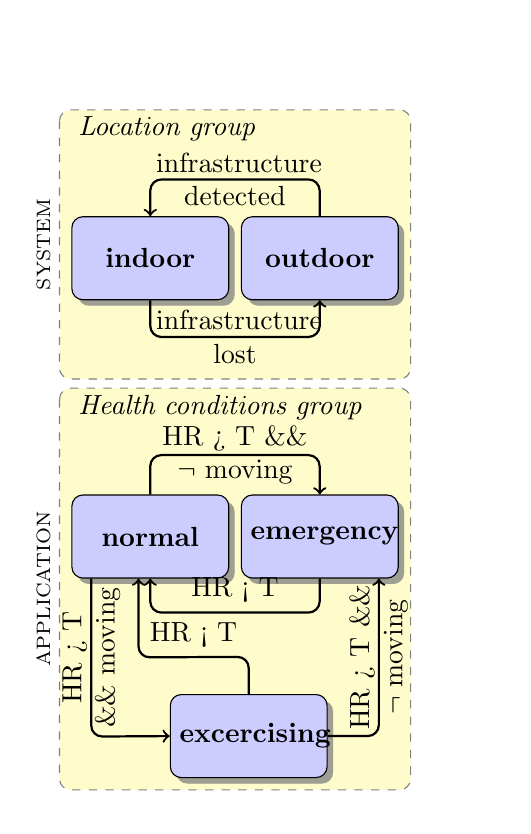
\begin{tikzpicture}
  \path \context{1}{indoor};
  \path (c1.east)+(1.15, 0.0) \context{2}{outdoor};
  \path (c1.south)+(0.0,-3) \context{3}{normal};
  \path (c3.south)+(1.25,-2.0) \context{5}{excercising};
  \path (c2.south)+(0.0, -3) \context{4}{emergency};
  \background{c1}{c1}{c2}{c1}{Location group}{SYSTEM}{-1}
  \background{c1}{c3}{c4}{c5}{Health conditions group}{APPLICATION}{-0.15}

  \draw [->, rounded corners, thick] (c1.south) -- (0,-1) -- (2.15,-1) node [midway,text width=2cm,align=center] {infrastructure\\lost} -- (c2.south);
  \draw [->, rounded corners, thick] (c2.north) -- (2.15,1) -- (0,1) node [midway,text width=2cm,align=center] {infrastructure\\detected}-- (c1.north);

  \draw [<-, rounded corners, thick] (c3.south) -- (0,-4.5) -- (2.15,-4.5) node [above,midway,text width=2cm,align=center] {HR < T} -- (c4.south);
  \draw [<-, rounded corners, thick] (c4.north) -- (2.15,-2.5) -- (0,-2.5) node [midway,text width=2cm,align=center] {HR > T \&\& $\neg$ moving}-- (c3.north); 

  \draw [->, rounded corners, thick] (c3.south)+(-0.75,0) -- (-0.75,-6.075) node [rotate = 90,midway,text width=2cm,align=center] {HR > T \&\& moving} -- (c5.west);  
  \draw [->, rounded corners, thick] (c5.east) -- ($(c4.south)+(0.75,-2)$) -- ($(c4.south)+(+0.75,0)$) node [rotate = 90,midway,text width=2cm,align=center] {HR > T \&\& $\neg$ moving}; 
  
  \draw [->, rounded corners, thick] (c5.north) -- ($(c5.north)+(0,0.471)$) -- ($(c3.south)+(-0.15,-1)$) node [above,midway,text width=2cm,align=center] {HR < T} -- ($(c3.south)+(-0.15,0)$);
      \end{tikzpicture}
\end{minipage}
 \caption{Sample}
 \label{fig:diagram}
\end{figure}
}

For a preliminary evaluation we also implemented two simple applications with the same functionality: by using {\textlst{ConesC}} and by using {\textlst{nesC}}. The binary of a program written using {\textlst{ConesC}} is only 2\% bigger than the binary of the program written using {\textlst{nesC}}: 7758 bytes vs 7640 bytes.

\balance
\bibliographystyle{acm-sigchi}
\bibliography{ubicomp}

\end{document}
